%mark = star, diamond, square, otimes
%\documentclass{article}
%\usepackage{pgfplots}
%\usepackage[justification=centering]{caption}
%\pgfplotsset{compat=newest}
%\begin{document}
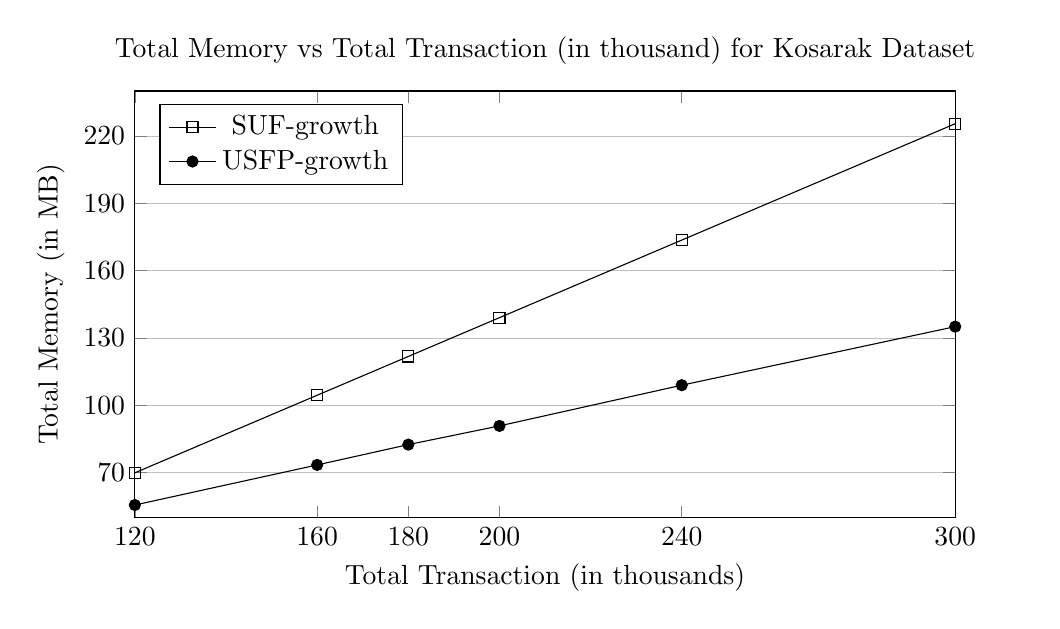
\begin{tikzpicture}
\begin{axis}[
	title={\parbox{\linewidth}{\centering Total Memory vs Total Transaction (in thousand) for Kosarak Dataset}},
	width=12cm,
	height=7cm,
    xlabel={Total Transaction (in thousands) },
    ylabel={Total Memory (in MB) },
    xmin=120, xmax=300,
    ymin=50	, ymax=240,
    xtick={120,160,180,200,240,300},
    ytick={70,100,130,160,190,220},
    legend pos=north west,
    ymajorgrids=true,
    grid style={line width=.2pt,draw=gray!50},
]
 
\addplot[
    solid, every mark/.append style={solid, fill=gray}, mark=square
    ]
    coordinates {
			(120,	69.945)
			(160,	104.492)
			(180,	121.766)
			(200,	139.039)
			(240,	173.587)
			(300,	225.408)

	};
    \addlegendentry{SUF-growth}
\addplot[
    solid, every mark/.append style={solid, fill=black}, mark=*
    ]
    coordinates {
			(120,	55.607)
			(160,	73.456)
			(180,	82.507)
			(200,	90.835)
			(240,	108.960)
			(300,	135.042)

};
    \addlegendentry{USFP-growth}
 
\end{axis}
\end{tikzpicture}
%\end{document}